\section{Decoders Management}

Selecting "Decoders" from the navigation drawer displays the main Decoders management view. This page displays a tabular listing of all Digital Command Control (DCC) decoders installed in inventory locomotives, summarizing information such as Road Name, Road Number, Manufacturer, Family, Model, active DCC Address, and available action controls. Figure \ref{fig:decoders} shows the main Decoders table page.

\begin{figure}[H]
    \centering
    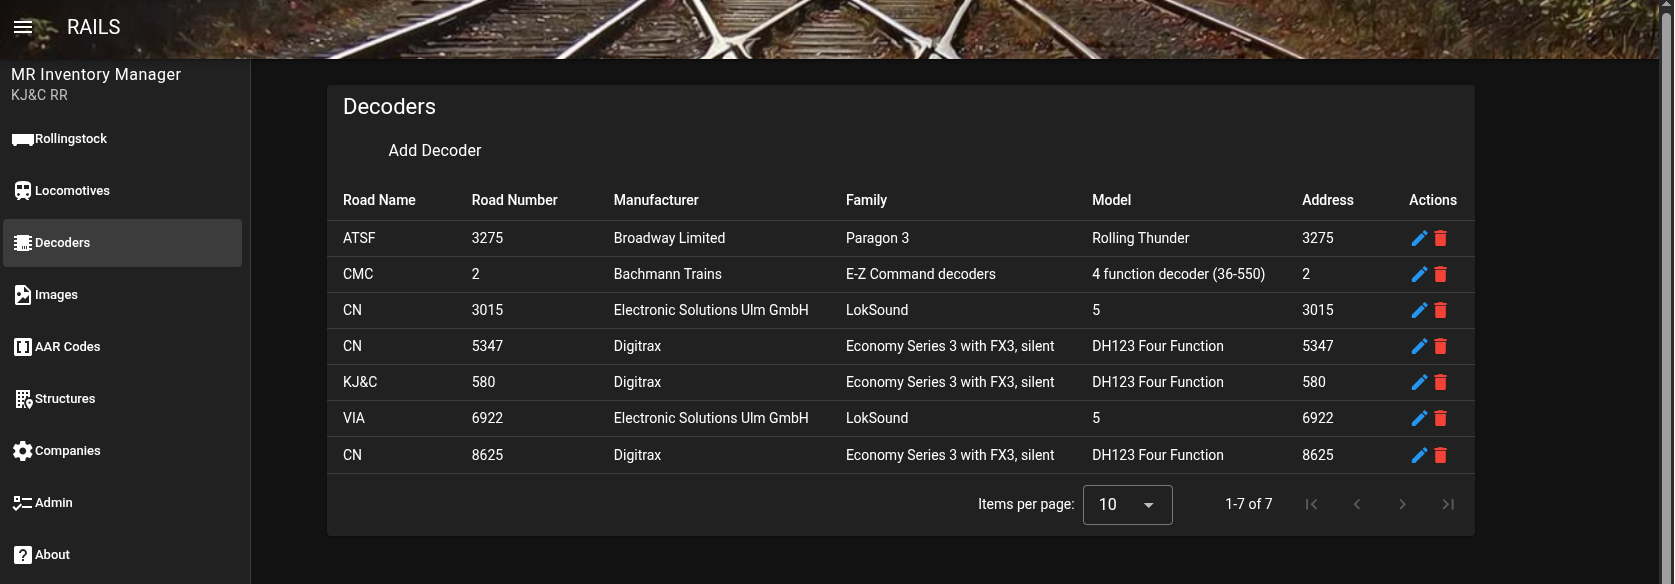
\includegraphics[width=0.85\textwidth]{./images/decoders.png}
    \caption{Decoders Page}
    \label{fig:decoders}
\end{figure}

\subsection{Adding a New Decoder}

Clicking the "Add Decoder" button above the table opens a modal dialog for registering a new decoder entry. The form includes fields for Road Name, Road Number, Manufacturer, Family, Model, and DCC Address. Figure \ref{fig:decoders-new} shows the new decoder entry dialog.

\begin{figure}[H]
    \centering
    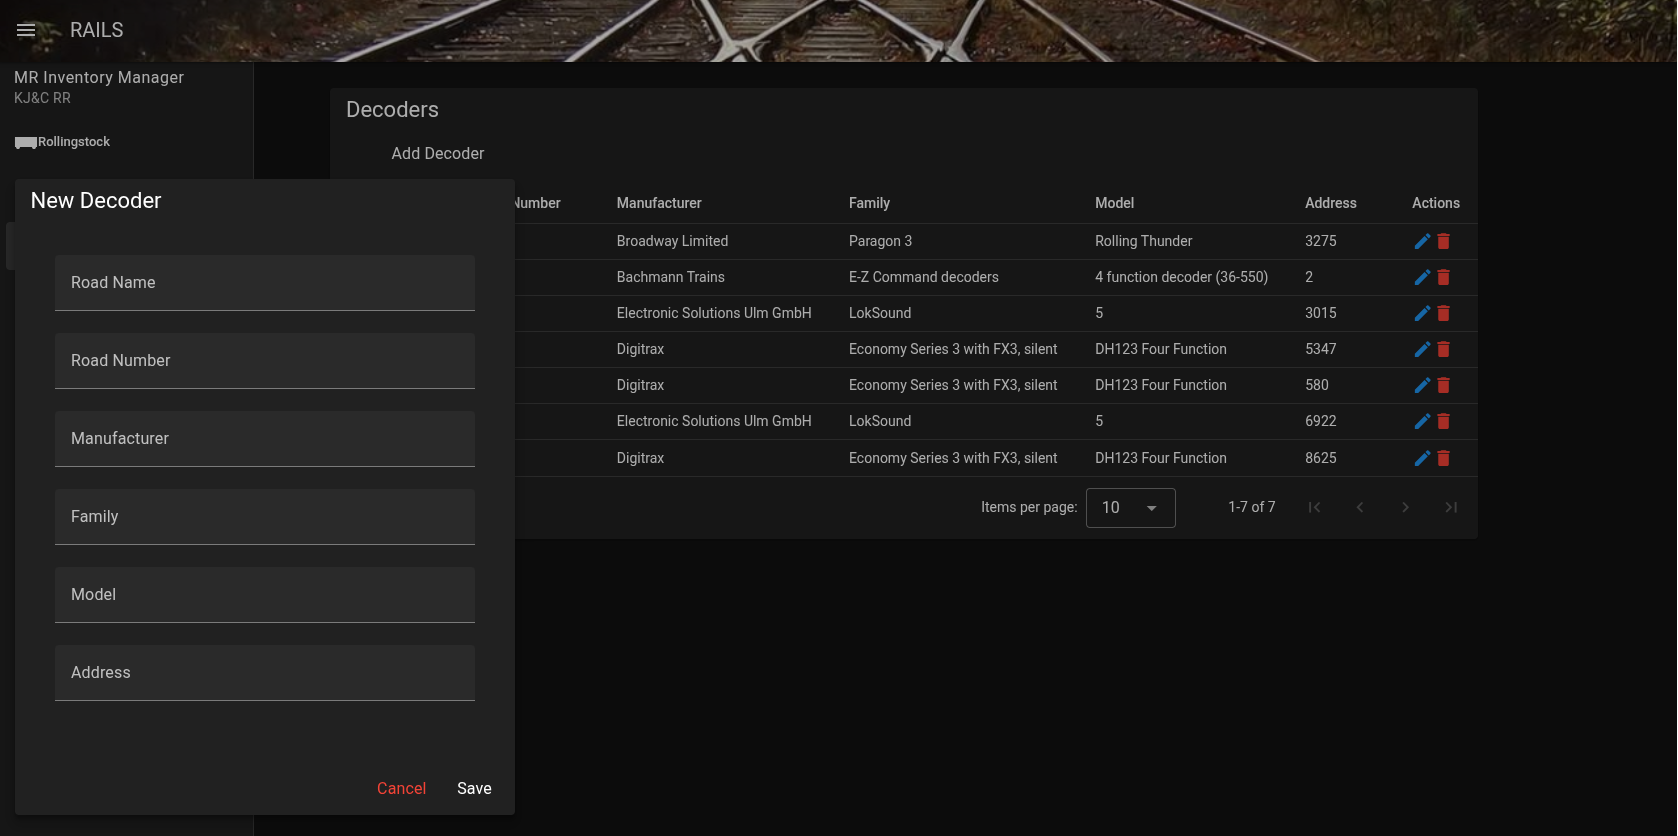
\includegraphics[width=0.85\textwidth]{./images/decoders-new.png}
    \caption{Add Decoder}
    \label{fig:decoders-new}
\end{figure}

\subsection{Editing Decoder Records}

To modify an existing decoder entry, click the blue pencil icon under the Actions column. This opens the decoder configuration form pre-populated with current settings, allowing updates to hardware details or DCC address assignments. Figure \ref{fig:decoders-edit} displays the edit decoder interface.

\begin{figure}[H]
    \centering
    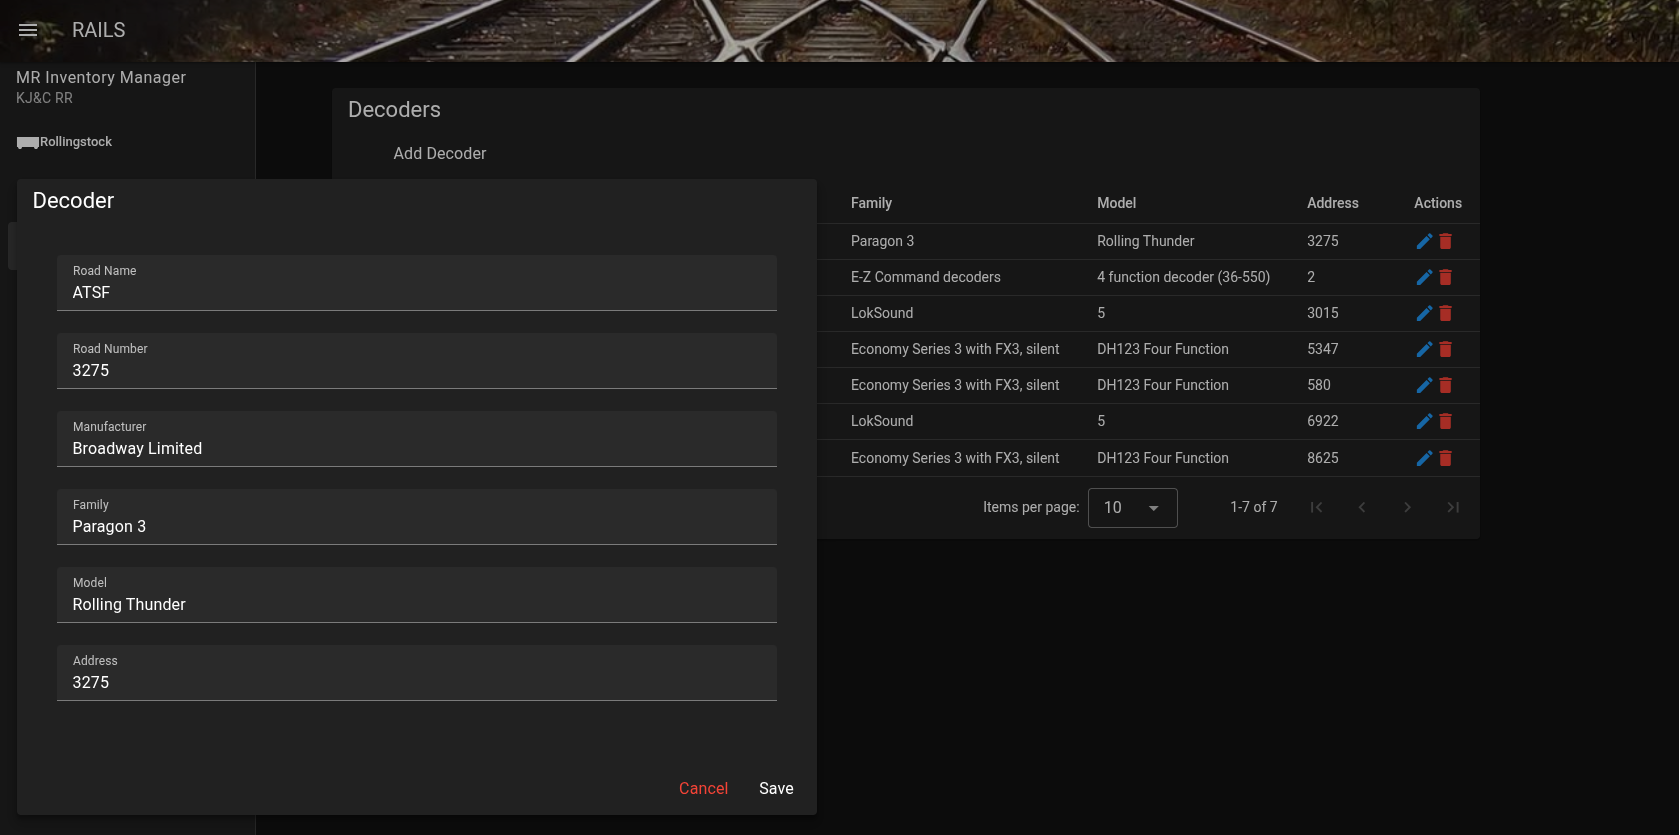
\includegraphics[width=0.85\textwidth]{./images/decoders-edit.png}
    \caption{Edit Decoder}
    \label{fig:decoders-edit}
\end{figure}

\subsection{Deleting Decoder Records}

To delete a decoder entry, click the red trash bin icon in the Actions column. A modal confirmation prompt appears requesting verification before the record is permanently removed from the database. Figure \ref{fig:decoders-delete} illustrates the deletion confirmation dialog.

\begin{figure}[H]
    \centering
    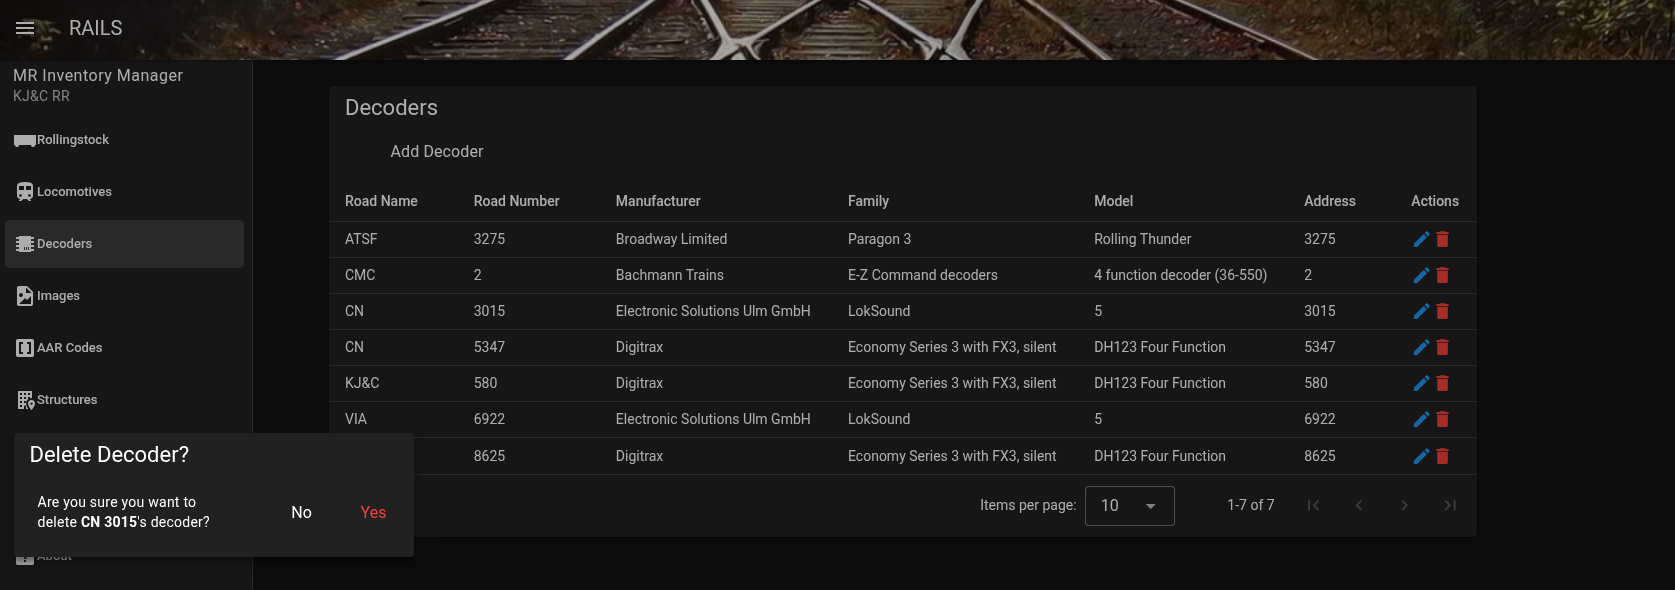
\includegraphics[width=0.85\textwidth]{./images/decoders-delete.png}
    \caption{Delete Decoder Confirmation}
    \label{fig:decoders-delete}
\end{figure}
